\chapter{Levelaufbau}
Das Level wird durch ein Skript (BattlefieldCreator) aufgrund der Plane generiert. Je gr"o"ser der Localscale der Plane, desto gr"o"ser wird
das Level. Auf einer Skalierung von 1/1/1 entsteht ein 10 * 10 Grid aus Quads(Zellen). Bei Skalierungen im Komma Bereich werden dem entsprechen viele Zellen erstellt. Zum Beispiel bei x = 1,6 und z = 1,7 entsteht ein 16 * 17 Feld.

\begin{lstlisting}[breaklines = true]
 //Initialisiert alle Zellen
 for (float z = 0; z > -(sizeZint); z--) {
	 for (float x = 0; x < (sizeXint); x++) {
		 GameObject zelle = GameObject.CreatePrimitive(PrimitiveType.Quad);
		 zelle.transform.Rotate(new Vector3(90, 0, 0));
		 zelle.AddComponent<Cell>();
		 zelle.tag = "Cell";
		 zelle.name = x + "|" + -z;
		 zelle.transform.position = new Vector3((x + 0.5f), 0.001f, (z - 0.5f));
\end{lstlisting}

Die Objekte werden durch das Skript ObjectSetter beim Spielstart auf dem Grid platziert. Sollte ein Objekt gr"o"ser als eine Zelle sein so wird dies in der ObjectComponent durch X und Z wert angegeben. Ebenso wird dort vermerkt ob das Objekt Deckung bietet und die Zelle besetzt.


\begin{figure}
	\centering
	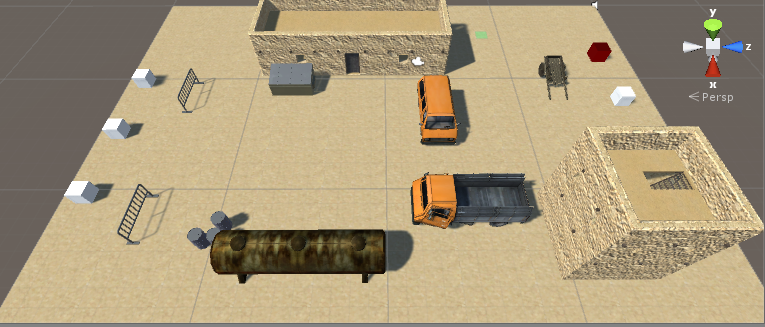
\includegraphics[height=6cm]{images/FinalLevel.png}
	\caption{Das finale Level mit Spieleraufstellung}
	\label{fig:FinalLevel}
\end{figure}